
\addcontentsline{toc}{section}{Repository for the code : R Package}
\subsection*{Repository for the code : R Package}

An \textbf{R package} has been created and can be easily downloaded from its \textbf{repository} :
\begin{center}\label{xxx}
 \url{https://github.com/proto4426/PissoortThesis}
\end{center}
by following the instructions in the README. It follows the standard structure of an usual R package (see e.g. \citet{leisch_creating_2008}) and make use of the \texttt{roxygen2} package for the documentation.

For your (best?) convenience, an external folder has been created in this repository containing all the scripts created during this thesis. It allows to reproduce all the results, and sometimes with more details, tables or plots. It can be retrieved directly by going into the \textbf{/Scripts-R/} folder from the repository. We will notice in the beginning of each of the following chapter to which script(s) it corresponds. We also explain in more details the structure of the github repository in \hyperref[appgit]{appendix \textbf{\ref{appgit}}} to give you a better idea of what each folder and each file is about.

\addcontentsline{toc}{subsection}{Visualization Tool : Shiny Application}
\subsection*{Visualization Tool : Shiny Application}

A small Shiny application has started to be developed and can be run directly from R after having the package loaded in your environment, by only typing 

\begin{center}
\begin{lstlisting}[language=R]
runExample()  # in the R console. Then, choose the propositions displayed
\end{lstlisting}
\end{center}
and write it in (). So far, it contains an application based on figure \ref{gevdens} from which you can visualize the GEV distribution and the influence of the parameters ('GEV\_distributions'). There are also applications dedicated to the annual maxima that can you can smoothly visualize and an application for the simulations of the GAM model with splines and the coverage visualization (\hyperref[sec:firstana]{section \textbf{\ref{sec:firstana}}}).  Actually, it summarizes the contents of figure \ref{first_fig} It was difficult to do more because we could not publicly disclose the datasets provided by the IRM.



The following analysis relies on \texttt{1inter\_stationary.R} and \texttt{1intro\_trends(splines).R} codes from the \textbf{/Scripts-R/} folder of the github repository.

\section{Presentation of the Analysis : Temperatures from Uccle}

The data used during this thesis have been gathered directly from the "Institut Royal de Météorologie" (IRM). We were provided data...


\subsection{Open shelter vs Closed shelter}

For\textbf{ meteorological considerations}, it is better to consider temperature's analysis in \textbf{closed shelters}, following for example \citet{lindsey_use_1956}. Indeed, and thanks to grateful advices from mr Tricot working for the IRM : 
\begin{itemize}
	\item It can
	\item It
\end{itemize}


\subsection{Comparisons with freely available data} 

A similar dataset is freely available on the internet\footnote{\url{http://lstat.kuleuven.be/Wiley/Data/ecad00045TX.txt}}. It was a project initially performed by the KMNI and which was used for example in \citet{beirlant_statistics_2006}. However, we were reticent to simply analyze these data as we know that it is hard to trust internet's data, even if they come from well-known "authorities". After having made all these comparisons analysis (see start of code...), we remark effectively that there are differences
in these two datasets, and hence large errors of measures can easily occur 
in unofficial data. It confirms the fact that is important to get reliable data if one wants to make reliable analysis. 
However, these differences tend to be much smaller when considering the "open shelter"
version ($54\%$ of equal measurements in closed shelter VS $14.4\%$ in the closed case). For this reason, we have confidence that this public datasets
is dealing with open shelter temperatures data.






\section{First Analysis : Block-Maxima}\label{sec:firstana}


\subsection{Descriptive Analysis}

Taking yearly blocks leaves us with $n=116$ data which seem justifiable for further GEV analysis and the conditions to hold (see)


\subsection{First visualization with simple models}

We present our series of yearly maxima in figure \ref{first_fig} where we introduce 3 \textbf{models for the trend} :


\begin{figure}[!htb]
	\centering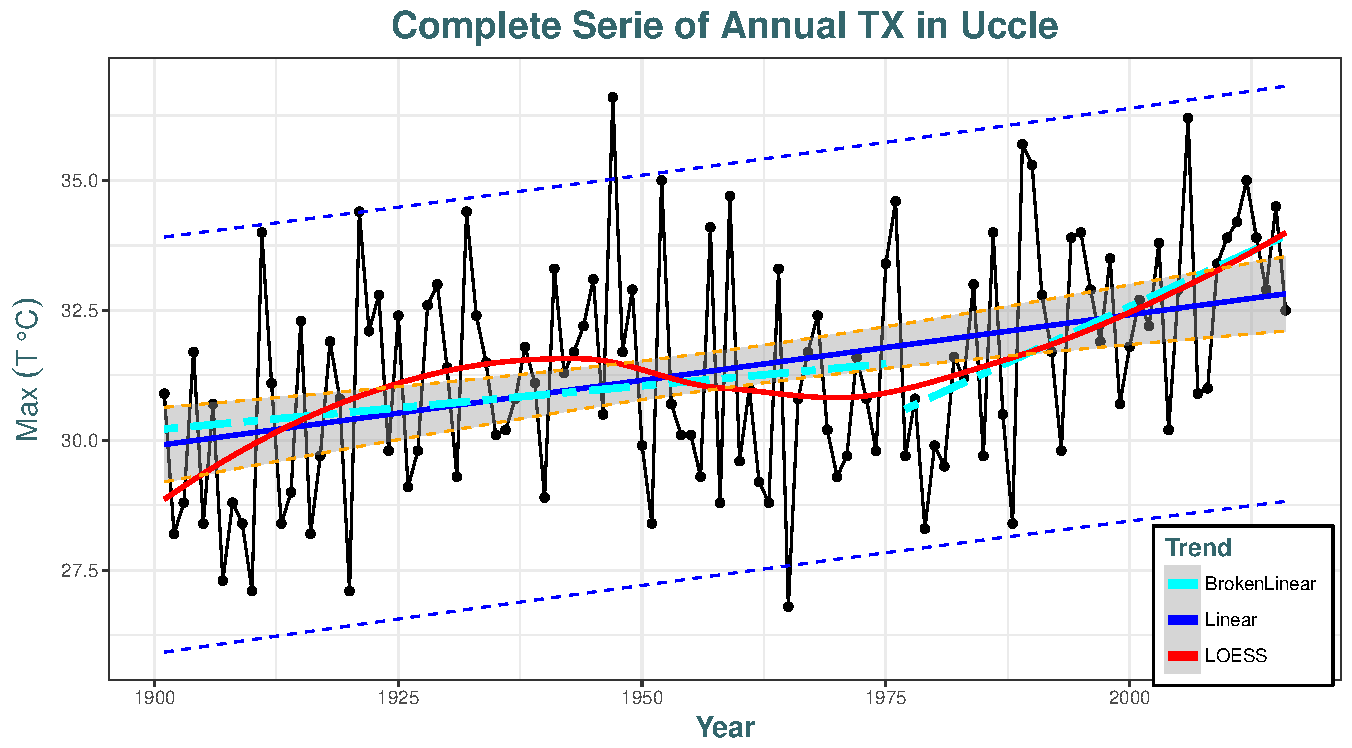
\includegraphics[width=.8\linewidth]{gg12.pdf}\caption{representing the \textbf{yearly} \textbf{maxima} together with three first models trying to represent the trend. Note that shaded grey line representing the standard errors (and not a confidence interval) of the linear trend.}\label{first_fig}
\end{figure}


\begin{itemize}
\item \emph{Linear regression } (in blue) which is a \textbf{parametric} fit. We remark that it is slightly but significantly increasing over time ($\text{p-value}\approx 10^{-5}$) . 
\item \emph{Local Polynomial regression } or LOESS (in red) which is a \textbf{nonparametric} fit. It tells us that the yearly maxima process is rather "dispersed". For example, the drop in the series visible around years 1950 to 1975 is probably due to a 'random effect' rather than a real decrease or freezing of the maximum temperatures at this time. Moreover, it will disappear if we change the parameter controlling the degree of smoothing. We will assess that more formally in the \hyperref[sec:splines]{next section}.
\item \emph{Broken-linear regression} (in cyan) which is a \textbf{parametric} fit. We wanted to emphasize visually the difference in trend between the period [1901-1975] and [1976-2016]. The two periods have been chosen arbitrarily and we will study that more formally in the \hyperref[sec:splines]{next section}.
\end{itemize}


The code which provide all the tools to retrieve the presented results are left in appendix, but in the numeric version only be cause it is very heavy. this also enables you to get all insights (..)



\subsection{Deeper Trend Analysis : Splines derivatives in GAM}\label{sec:splines}

Apart from the significant increasing linear trend, we did not find formal results. Moreover, we see from the series that a linear trend to the entire series makes little sense. Regarding the broken-linear trend for example, we would like to assess if there is indeed a difference in the slope of trend over time. 

We assume the reader is at ease(?) with\emph{ Generalized Additive Models} (GAM) which have been developed by \citet{hastie_generalized_1986}. We also assume he knows about penalized \emph{splines} and splines smoothing, where a good introduction is found in \citet[section 3]{ruppert_semiparametric_2003}. This section uses the code \textbf{/Scripts-R/1intro\_trends(splines).R}.


\addcontentsline{toc}{subsubsection}{Pointwise vs Simultaneous intervals}
\subsubsection*{Pointwise vs Simultaneous intervals}

\textbf{Simultaneous} confidence intervals :  Following \citet[section 3, section 4.9, section 6.5]{ruppert_semiparametric_2003} which uses a simulation-based approach to generate a simultaneous interval
\citet{marra_coverage_2012}

From the pointwise confidence intervals we can say that (example) $f(1980)$ has $95\%$ chance to lie within (-1,0) (say) and $f(2000)$ has also $95\%$ to lie within (0.2,1.2) BUT it is a fallacy to say simultaneously that both are contained in these intervals at the same time with $95\%$ confidence. \citet[section 6.5]{ruppert_semiparametric_2003}


\addcontentsline{toc}{subsubsection}{Methodology}
\subsubsection*{Methodology}

\begin{itemize}
\item We fitted a simple GAM model relying on the \texttt{mgcv} package from \citet{maindonald_data_2006}. Then, after looking at the correlation structure the normalized residuals (ACF and PACF, see figure \ref{fig:acfresgam1} in \hyperref[app:fig]{appendix \ref{app:fig}}), we detected very slight patterns.

\item As the selection from figure \ref{fig:acfresgam1} is not trivial, we fitted several time series models for the residuals. It is not necessary to consider too complex models so we stopped at 2 additional degrees of freedom. The results are represented in table \ref{table:gamresid} in \hyperref[app:fig]{appendix \ref{app:fig}} where we see that the BIC, which is more penalizing complex models, will prefer the independent model for the residuals but the AIC will not. Hence, we conducted likelihood ratio tests which confirmed. The diagnostics of the model in figure \ref{fig:diagnogam} are good. As we took a Gaussian (identity) link, our model can be written as

\begin{equation}\label{eq:gam}
Y_{\text{GAM}}(\text{year}) = \alpha + f_{\text{(k)}}(\text{year})+\epsilon , \qquad\quad \epsilon\sim\text{WN}.
\end{equation}

(!! WN or MA(1° for the residuals ? Depend on the analysis !!! Graph below is WN)


where $f$ is modelled by smoothing splines. $Y$ models the TX here. It is not important in our case to perform cross-validation to choose the dimension of the basis $k$ and we set it to 20 to ensure a reasonable degree of smoothness.

\begin{figure}[!htb]
\centering	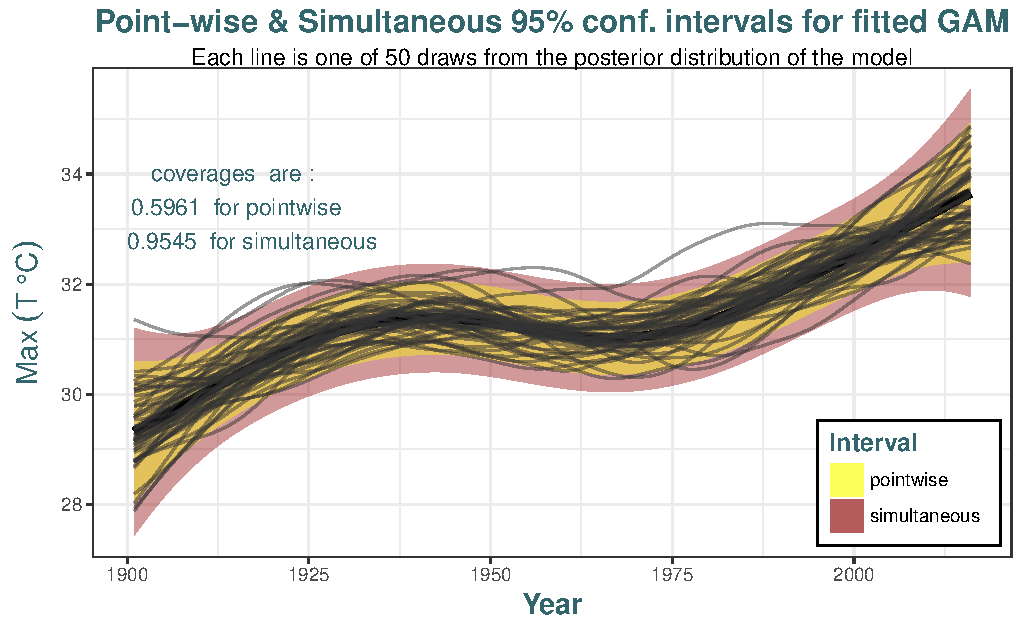
\includegraphics[width=.75\linewidth]{post_draws.pdf}\caption{displays draws from the posterior distribution of the model. Notice the large uncertainty associated to the posterior draws (grey lines).  The coverages are calculated for $M=10^5$ simulations. }\label{fig:post_draws}
\end{figure}

\item  To account for uncertainty, we decide to simulate $M = 10^5$ draws (it is quite fast) from the posterior of the GAM model in (\ref{eq:gam}). Hence, the confidence intervals (or bands) that we will compute will be of the form of  Bayesian credible intervals that we have discussed in \hyperref[bayes_cred_int]{section \textbf{\ref{bayes_cred_int}}}.
We display 50 of the posterior draws in figure \ref{fig:post_draws} %let in \hyperref[app:fig]{appendix \ref{app:fig}}
 displaying both pointwise (in yellow) and simultaneous (in red) intervals. We can already point out that pointwise intervals seem too narrow.

\end{itemize}

We can see the two significant increase in trend from figure \ref{fig:center_gam} let in \hyperref[app:fig]{appendix \ref{app:fig}}. The decrease we have pointed out in the preceding section with LOESS is hence not significant. However, we will now see more precisely that this is not the case when doing the correction for simultaneous intervals and compare the results. 


\subsubsection*{Coverage Analysis} 
We would like to formalize the inadequacy of the pointwise intervals. Hence, we computed posterior draws of the fitted GAM and we looked how many draws lie within each intervals.
\begin{table}[!htbp] \centering 
  \caption{Proportion of the $M$ posterior simulations which are covered by the confidence intervals} \label{tab:cov} 
\begin{tabular}{@{\extracolsep{5pt}}lccccc} 
\\[-1.8ex]\hline 
\hline \vspace{-.1cm}\\[-1.8ex] 
\textbf{Coverage at $95\%$} & \multicolumn{1}{c}{$M=20$} &  \multicolumn{1}{c}{$M=100$} & \multicolumn{1}{c}{$M=10^3$} & \multicolumn{1}{c}{$M=10^6$} \vspace{.1cm} \\ 
\hline \\[-1.8ex] 
\underline{Pointwise} & $40\%$ & $63\%$ & $61.1\%$ & $59.463\%$ \\
\underline{Simultaneous} & $80\%$ & $91\%$ & $94.9\%$ & $95.019\%$  \\
\hline \\[-1.8ex] 
\end{tabular} 
\end{table}

We clearly see that this indeed converges to $95\%$ for the simultaneous interval while it converges rather to $\approx 60\%$ for the pointwise interval.

We have build a Shiny application from this graph to better visualize the impact of the number simulations on the confidence intervals and how their coverage vary, both visually and quantitatively. You can load it from the package with \begin{lstlisting}[language=R]
runExample('splines_draws')\end{lstlisting} from which you can check the results of the table (using the default seed=99)

Note that the results are similar if we do the experiment on the first derivatives $f^{'}(\cdot)$ of the splines rather than on the splines itself


\addcontentsline{toc}{subsubsection}{Final Results}
\subsubsection*{Final Results}


Some remarks from the two plots in figure \ref{fig:derivsplines} :

\begin{figure}[!htb]
	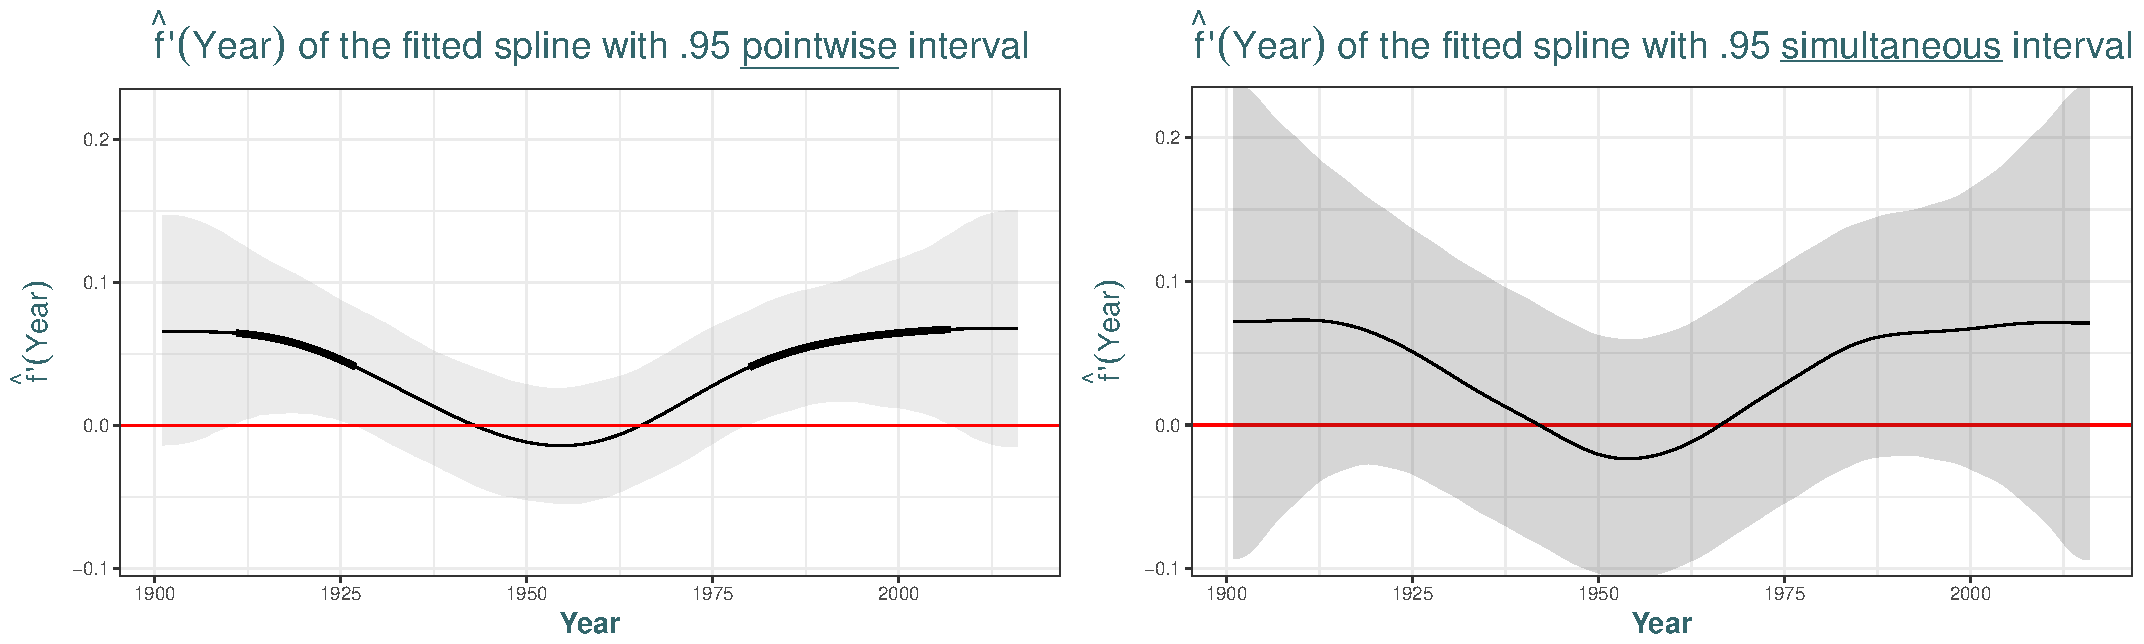
\includegraphics[width=.99\linewidth]{splines.pdf}\caption{Plots of the first derivative $f^{'}(\cdot)$ of the estimated splines on the retained GAM model. Grey area represents the $95\%$ confidence interval. Sections of the spline where the confidence interval does not include zero are indicated by thicker sections. }\label{fig:derivsplines}
\end{figure}

\begin{itemize}
\item Looking together with the series in \ref{first_fig}, we can make the link between the trend behaviour of the series and the splines derivative which models accurately the slope behaviour of the trend. 
\item Whence we can notice the increasing trend but with decreasing slope until $\approx 1945$ where it becomes is decreasing. Then the slope increase and the trend starts to re-increase around 1962. This upward trend that the series of annual maxima is facing for this last period brings light to the climate warming we are all talking about. However, 
\item  Whereas the pointwise confidence interval include significant regions (i.e. when 0 is not included in the interval), the simultaneous interval which accounting for the increase in uncertainty, have no more significant regions. We can concluce that the 

\end{itemize}


We can see that only the 2 increasing periods from the start and at the end of the series are significant, while the decreasing period from... (see the red line) is more likely to be the subject of randomness. Moreover, we remark that the 


\section{Comments and Structure of the Analysis }

 We have remarked that there is indeed an upward (linear) trend for the series of yearly maxima but which is not significant when doing the correction for simultaneous intervals.
We have then remarked that the \textbf{nonstationary} component is present. After having... we will now go through with the more specific subjec of this thesis, that is the extreme value analysis. Hence, after having presented a stationary analysis in \hyperref[sec:anagev]{section \ref{sec:anagev}}, we will make an in-depth nonstationary analysis in \hyperref[sec:ananonsta]{section \ref{sec:ananonsta}}.


POT and GEV : 
As you have seen, the analysis in POT or in GEV involves different methods and different data. For the kind of this text, we decide not to display the results of the POT analysis to keep the text not too enormous. Henceforth, we will be able to focus on the GEV analysis. But\textbf{ note that the analysis in POT have been done and are available on the same \hyperref[xxx]{github repository} presented above}.
\hyperref[appgit]{Appendix \ref{appgit}} summarize its contents.


Results are not shown here but this is (visually) less pronounced for minima. We have also conducted some analysis by dividing the dataset by seasons, by hot and cold months (July-August, January-February), ... 
Comparisons are interesting (and are also available on the repository) but this is not at the core of this text. 
We will then only \textbf{focus on a GEV analysis on yearly maxima}.